\subsubsection{Szukanie zbioru $k$-helpful gdzie $k \geq limit$}
Proces budowania zbiorów helpful pokazany jest na rysunku \ref{im:building-helpfulsets}(a).
Te zbiory nazywane są zbiorami Help.
Kardynalność tych zbiorów rośnie dynamicznie podczas szukania.
Dzięki temu, że podczas budowania zbioru Help aktualizujemy tylko wartości helpfulness wierzchołków z tej samej partycji,
obydwa zbiory Help mogą byc budowane niezależnie i równolegle.
Jednak w mojej implementacji (rysunek \ref{code:helpful_sets}) budowane są one jeden po drugim
(jeśli warunek pozwoli na zbudowanie drugiego).

Podczas tego procesu brane pod uwagę są tylko wierzchołki z wartością helpfulness $\geq$ $0$.
Może to prowadzić do przedwczesnego zakończenia wywołania algorytmu, jeśli żadne wierzchołki z taką wartością
helpfulness nie będą już dostępne, ale to także gwarantuje, że wartość helpfulness dla zbioru Help nigdy nie będzie
maleć.
Wyszukiwanie zbioru Help kończy się, gdy jego wartość helpfulness osiąga \texttt{limit} lub jeśli nie ma więcej wierzchołków
z wartością helpfulness $\geq$ $0$.

Po udanym wywołaniu, zbiór $S$, który jest zbiorem Help z większą wartością helpfulness, przenoszony jest
na drugą stronę podziału.
Drugi zbiór Help jest usuwany i nie jest więcej brany pod uwagę.
Na rysunku \ref{im:building-helpfulsets}(b) BIG SET reprezentuje $V_1$ lub $V_2$ połączone z $S$.
SMALL SET to pozostała część, która została zredukowana o $S$.
\begin{figure}[h]
\begin{subfigure}{.5\textwidth}
    \centering
    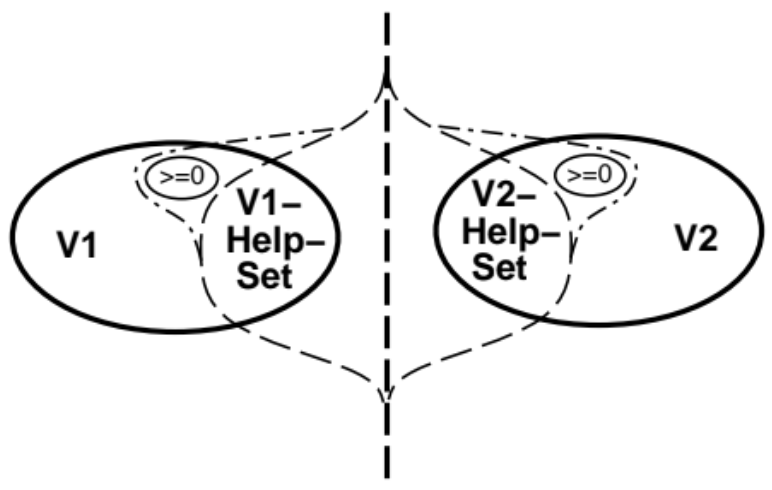
\includegraphics[width=0.8\textwidth]{images/building-helpfulsets/1}
    \caption[short]{}
\end{subfigure}
\begin{subfigure}{.5\textwidth}
    \centering
    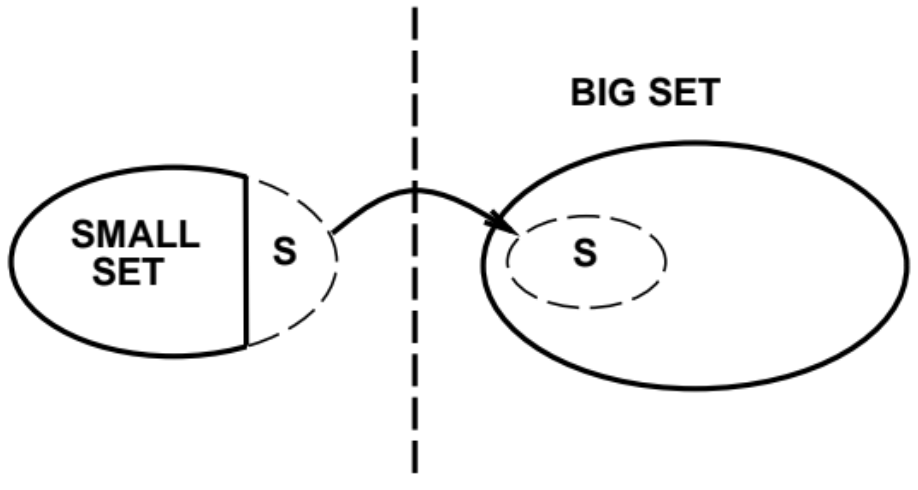
\includegraphics[width=0.8\textwidth]{images/building-helpfulsets/2}
    \caption[short]{}
\end{subfigure}%
\caption{Szukanie zbioru $k$-helpful poprzez przenoszenie wierzchołków z wartością helpfulness $\geq$ $0$
do zbiorów Help (a). (b) to przenoszenie zbioru $S$ na drugą stronę podziału.
Źródło: \cite{article}.}
\label{im:building-helpfulsets}
\end{figure}